\documentclass[a4paper, 12pt]{article}

\usepackage[left=2cm,right=2cm,
top=2cm,bottom=2cm,bindingoffset=0cm]{geometry}

\usepackage[T2A]{fontenc}
\usepackage[utf8]{inputenc}
\usepackage{color}
\usepackage{graphicx}
\usepackage{caption}
\usepackage{subcaption}
\usepackage{tikz}
\usepackage[english, russian]{babel}
\usepackage{ gensymb }
\usepackage{booktabs}
\usepackage{amsmath,amsfonts,amssymb,amsthm,mathtools}
\usepackage{lscape}
\usepackage{float}
\usepackage{pdflscape}
\usepackage{array}
\usepackage{multirow}
\usepackage{gensymb}
\usepackage{ wasysym }
\usepackage{listings}

\begin{document}	
	\begin{center}
		\textit{\textbf{Задача }}
	\end{center}
	
	К закрепленному в стене концу стержня $(x=0)$ подводится тепловой поток
	интенсивности q. На свободном конце стержня $(x=L)$ происходит конвективный
	теплообмен тепла. Коэффициент теплообмена $h$, температура окружающей среды $T_{cp}$.
	Через боковую поверхность стержня также происходит конвективный теплообмен.
	Площадь поперечного сечения стержня $S$ считается постоянной.
	
	Решить задачу методом конечных элементов с использованием одномерного
	линейного (симплекс) элемента. Выписать в тетради явное решение СЛАУ в случае
	когда стержень разбит на 3 элемента.
	
	Разбить стержень на 5 конечных элементов и вычислить температуру в узлах МКЭ
	запрограммировав на языке С++.
	
	Решить задачу при следующих данных:
	
	$k_x=75\left[\text{Вт/(см)}\cdot \celsius \right]$ - коэффициент теплопроводности материала, 
	
	$q=-150\left[\text{Вт/}\text{см}^2 \right]$ - считается, что положительное направление, когда тепло отводится от тела, так как по задаче тепло подводится, то знак минус
	
	$\alpha_g=10\left[\text{Вт/}\text{(см)}^2\cdot \celsius \right]$ - коэффициент теплообмена, $S=\pi \text{см}^2, L=7.5\text{ см}$
	

	\begin{figure}[h]
		\centering
		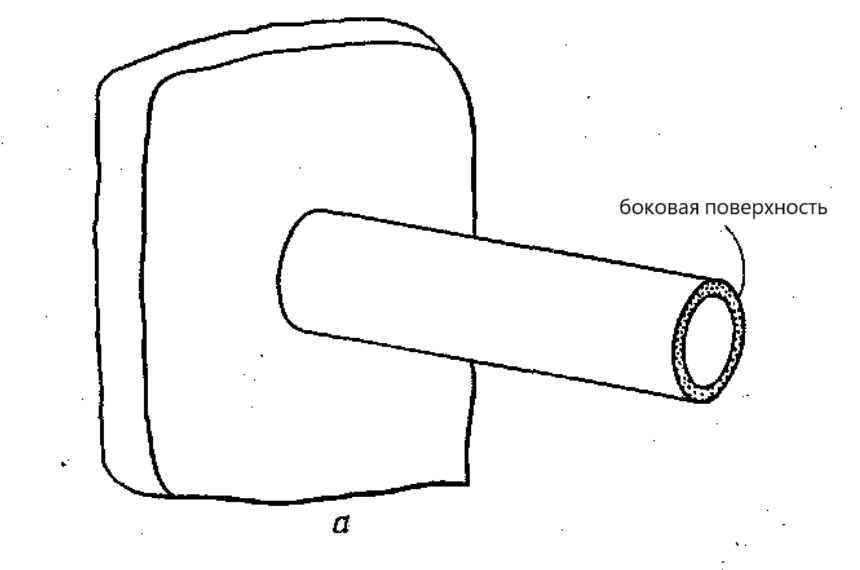
\includegraphics[width=0.5\textwidth]{task.png}
	\end{figure}
	
	\begin{center}
		\textbf{\textit{Решение}}
	\end{center}
	
	\textbf{1.} Дискретизация области одномерными элементами и границы:
	\begin{figure}[h]
		\centering
		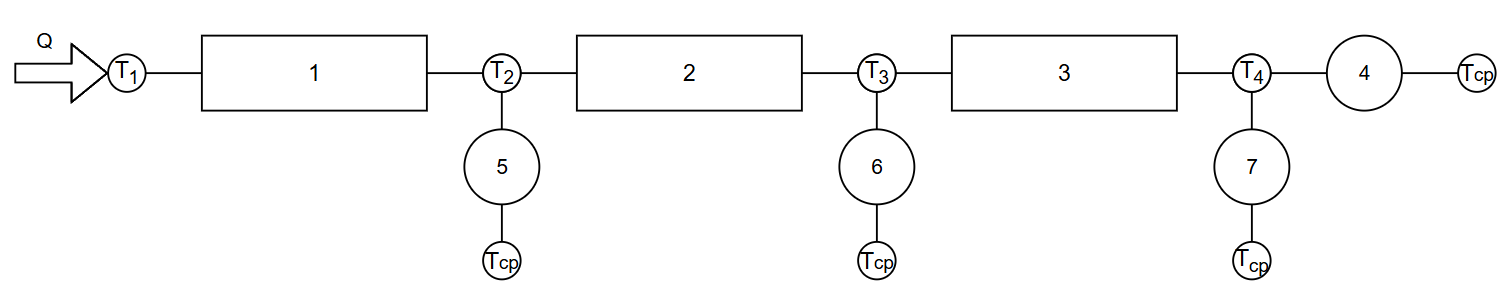
\includegraphics[width=1\textwidth]{graph1.png}
	\end{figure}
	\begin{figure}[H]
		\centering
		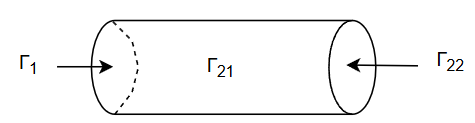
\includegraphics[width=0.4\textwidth]{graph2.png}
	\end{figure}
	
	Рассмотрим дифференциальное уравнение, описывающее распространение тепла в
	стержне: 
	\[
	-\frac{d}{dx}(k_x\frac{dT}{dx})=f \tag{1}
	\]

	где $f$ - погонная интенсивность подачи тепла, если внутри стержня есть источник. В задаче внутренние источники тепла не заданы, следовательно, $f=0$.
	
	Граничные условия:
	\[
	Q_1=k_x\frac{dT}{dx} \bigg{|}_{x=0} =-q; \qquad 	Q_2=k_x\frac{dT}{dx} \bigg{|}_{x=L} =\alpha_g(T_{cp}-T(l)) \qquad 	Q_2=k_x\frac{dT}{dx} \bigg{|}_{\Gamma} =\alpha_g(T_{cp}-T)
	\]\\


	Вычисления:
	\[
	A\cdot \Phi = P
	\]
	\[
	A=\int\limits_VB^TKB\ dV + \int\limits_{\Gamma_2} \alpha_g N^TN\ dS = \underbrace{k_x\cdot S \int\limits_{x_i}^{x_{i+1}} B^TB\ dx}_{\Gamma_1} + \underbrace{2\pi R \int\limits_{x_i}^{x_{i+1}} \alpha_g N^TN\ dx}_{\Gamma_{21}} +\underbrace{\alpha_g\cdot S \cdot \begin{bmatrix}
			0&0\\0&1
	\end{bmatrix}}_{\Gamma_{22}}=\astrosun
	\]
	\[
	\int\limits_{x_i}^{x_{i+1}} B^TB\ dx = \frac{1}{l}\begin{bmatrix}
		1&-1\\-1&1
	\end{bmatrix}
	\]
	\[
	\int\limits_{x_i}^{x_{i+1}} N^TN\ dx = \frac{l}{6}\begin{bmatrix}
		2&1\\1&2
	\end{bmatrix}
	\]
	\[
	\astrosun = \frac{k_x S}{l}\begin{bmatrix}
		1&-1\\-1&1
	\end{bmatrix}+\frac{\pi R l \alpha_g}{3}\begin{bmatrix}
	2&1\\1&2
	\end{bmatrix}+\alpha_gS \cdot \begin{bmatrix}
	0&0\\0&1
	\end{bmatrix}
	\]
	\[
	P=\int\limits_{\Gamma_1}N^T q\ dS +\int\limits_{\Gamma_2} \alpha_g T_g N^T \ dS = \underbrace{qS\begin{bmatrix}
			1\\0
	\end{bmatrix}}_{\Gamma_1}+\underbrace{l\pi R	\int\limits_{x_i}^{x_{i+1}} \alpha_g T_g N^T dx}_{\Gamma_{21}}+\underbrace{\alpha_g T_g S\begin{bmatrix}
	0\\1
\end{bmatrix}}_{\Gamma_{22}}
	\]
	
	СЛАУ:
	\[
	i=1: \begin{bmatrix}
		\dfrac{k_xS}{l}+\dfrac{2\pi R \alpha_g l}{3} & -\dfrac{k_xS}{l}+\dfrac{\pi R \alpha_g l}{3} \\ & \\
		-\dfrac{k_xS}{l}+\dfrac{\pi R \alpha_g l}{3} & \dfrac{k_xS}{l}+\dfrac{2\pi R \alpha_g l}{3} 
	\end{bmatrix} \begin{bmatrix}
	T_1\\ \\T_2
	\end{bmatrix}=\begin{bmatrix}
	qS+\pi R \alpha_g T_g l \\ \\
	\pi R \alpha_g T_g l
	\end{bmatrix}
	\]
	\[
	i=2: \begin{bmatrix}
		\dfrac{k_xS}{l}+\dfrac{2\pi R \alpha_g l}{3} & -\dfrac{k_xS}{l}+\dfrac{\pi R \alpha_g l}{3} \\ & \\
		-\dfrac{k_xS}{l}+\dfrac{\pi R \alpha_g l}{3} & \dfrac{k_xS}{l}+\dfrac{2\pi R \alpha_g l}{3} 
	\end{bmatrix} \begin{bmatrix}
		T_2\\ \\T_3
	\end{bmatrix}=\begin{bmatrix}
		\pi R \alpha_g T_g l \\ \\
		\pi R \alpha_g T_g l
	\end{bmatrix}
	\]
	\[
	i=3: \begin{bmatrix}
		\dfrac{k_xS}{l}+\dfrac{2\pi R \alpha_g l}{3} & -\dfrac{k_xS}{l}+\dfrac{\pi R \alpha_g l}{3} \\ & \\
		-\dfrac{k_xS}{l}+\dfrac{\pi R \alpha_g l}{3} & \dfrac{k_xS}{l}+\dfrac{2\pi R \alpha_g l}{3} +S\alpha_g 
	\end{bmatrix} \begin{bmatrix}
		T_3\\ \\T_4
	\end{bmatrix}=\begin{bmatrix}
		\pi R \alpha_g T_g l \\ \\
		\pi R \alpha_g T_g l + \alpha_g T_g S
	\end{bmatrix}
	\]
	
	Сделаем замену: 
	\[
	k_1=	\dfrac{k_xS}{l}+\dfrac{2\pi R \alpha_g l}{3} \qquad k_2= 	-\dfrac{k_xS}{l}+\dfrac{\pi R \alpha_g l}{3} \qquad p_1=\pi R \alpha_g T_g l
	\]
	
	Тогда:
	\[
	\begin{bmatrix}
		k_1&k_2&0&0 \\ k_2&2k_1&k_2&0\\ 0&k_2&2k_1&k_2\\ 0 & 0 & k_2  & k_1+S\alpha_g
	\end{bmatrix}\begin{bmatrix}
	T_1\\T_2\\T_3\\T_4
	\end{bmatrix}=\begin{bmatrix}
	qS+p_1\\2p_1\\2p_1\\p_1+\alpha_g T_g S
	\end{bmatrix}
	\]
	
	Конкретные значения:
	\[
	\begin{bmatrix}
		146.6&-68&0&0 \\ -68&293.2&-68&0\\ 0&-68&293.2&-68\\ 0 & 0 & -68  & 178
	\end{bmatrix}\begin{bmatrix}
		T_1\\T_2\\T_3\\T_4
	\end{bmatrix}=\begin{bmatrix}
		2435\\3926\\3926\\2748
	\end{bmatrix} \Rightarrow \Phi = \begin{bmatrix}
	28.6 \\ 25.9 \\25.2 \\25.1
	\end{bmatrix}
	\]
	
	Для пяти элементов построения и вычисления аналогичные, результат:
	\[
	\Phi = \begin{bmatrix}
		28.8 \\ 26.7 \\25.8 \\25.4 \\25.2\\25.1
	\end{bmatrix}
	\]
	
	Код для трех элементов:
	\begin{lstlisting}[language=Python]
	import math
	import numpy as np
	kx = 75
	q = 150
	alpha = 10
	S = math.pi
	L = 7.5
	R = 1
	Tg = 25
	n = 3
	l = L / 3
	k1 = (kx * S) / l + 2 * math.pi * R * alpha * l / 3
	k2 = -(kx * S) / l + math.pi * R * alpha * l / 3
	p1 = math.pi * R * alpha * Tg * l
	K = np.array(
		[
		[k1, k2, 0, 0],
		[k2, 2 * k1, k2, 0],
		[0, k2, 2 * k1, k2],
		[0, 0, k2, k1 + S * alpha],
		]
	)
	P = np.array([q * S + p1, 2 * p1, 2 * p1, p1 + alpha * Tg * S])
	L1 = np.linalg.cholesky(K)
	y = np.linalg.solve(L1, P)
	T = np.linalg.solve(L1.T, y)
	print(T)
	\end{lstlisting}
	
	\newpage
	Код для пяти элементов (матрица $K_1 = const$, матрица $K_2$ зависит от ГУ):
	\begin{lstlisting}
	n = 5
	l = L / n
	k1 = (kx * S) / l
	K1 = np.zeros((n + 1, n + 1))
	for i in range(n):
	K1[i, i] += k1
	K1[i, i + 1] = -k1
	K1[i + 1, i] = -k1
	K1[i + 1, i + 1] += k1
	print(np.round(K1, 3))
	k2 = math.pi * R * alpha * l / 3
	K2 = np.zeros((n + 1, n + 1))
	for i in range(n):
		K2[i, i] += k2 * 2
		K2[i, i + 1] = k2
		K2[i + 1, i] = k2
		K2[i + 1, i + 1] += k2 * 2
		K2[-1, -1] += S * alpha
	print(np.round(K2, 3))
	K = K1 + K2
	print(np.round(K, 3))
	p1 = math.pi * R * alpha * Tg * l
	P = np.zeros(n + 1)
	P[0] = q * S + p1
	for i in range(1, n):
		P[i] = 2 + p1
	P[-1] = p1 + alpha * Tg * S
	print(np.round(P, 3))
	L1 = np.linalg.cholesky(K)
	y = np.linalg.solve(L1, P)
	T = np.linalg.solve(L1.T, y)
	print(T)
	\end{lstlisting}
\end{document}